\mysection{Learning to Attend for Tracking}



The model is optimised for the following three objectives.
\begin{description}[leftmargin=\parindent,labelsep=1em]
	
	\item[Main Tracking Objective:] Maximise the overlap of predicted box with the true object.
	
	\item[Spatial Attention:] The glimpse should contain the object, but shouldn't be too big.
	
	\item[Appearance Attention:] The dynamic appearance features should respond specifically to the target object.
	
	
\end{description}


\vspace{.5\baselineskip}
\centering
\begin{minipage}[c]{.4\textwidth}
    \centering
    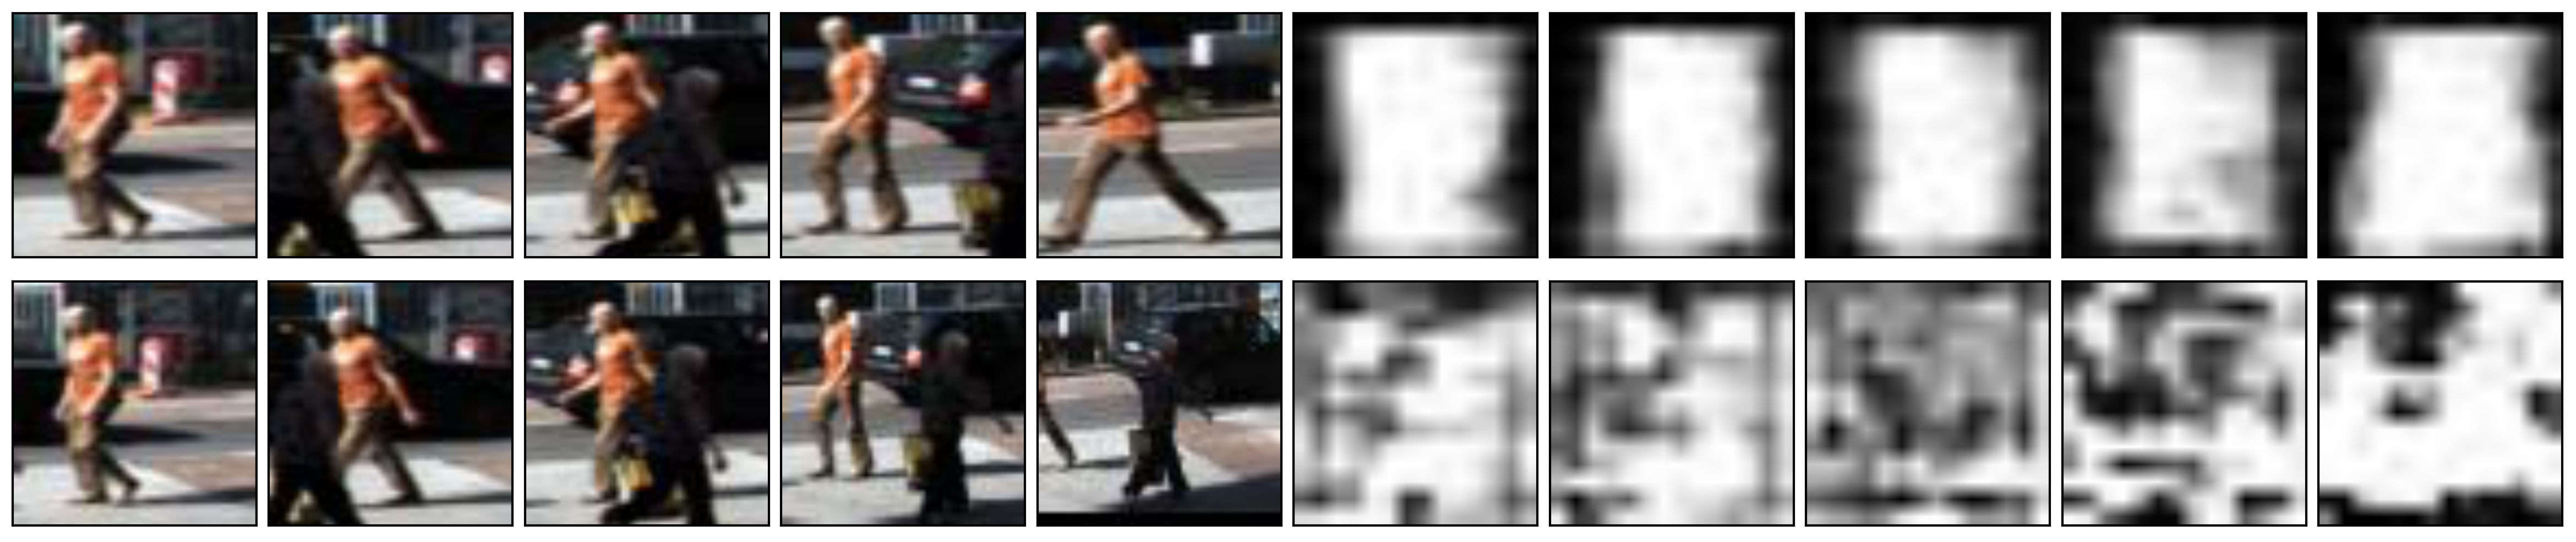
\includegraphics[width=\textwidth]{soft_id_swap}
%    \vspace{.2\baselineskip}
    \caption*{\large Appearance attention loss (top) prevents an ID swap when a pedestrian is occluded by another one (bottom).}
\end{minipage}
\begin{minipage}[c]{.4\textwidth}
    \centering
%    \vspace{.5\baselineskip}
    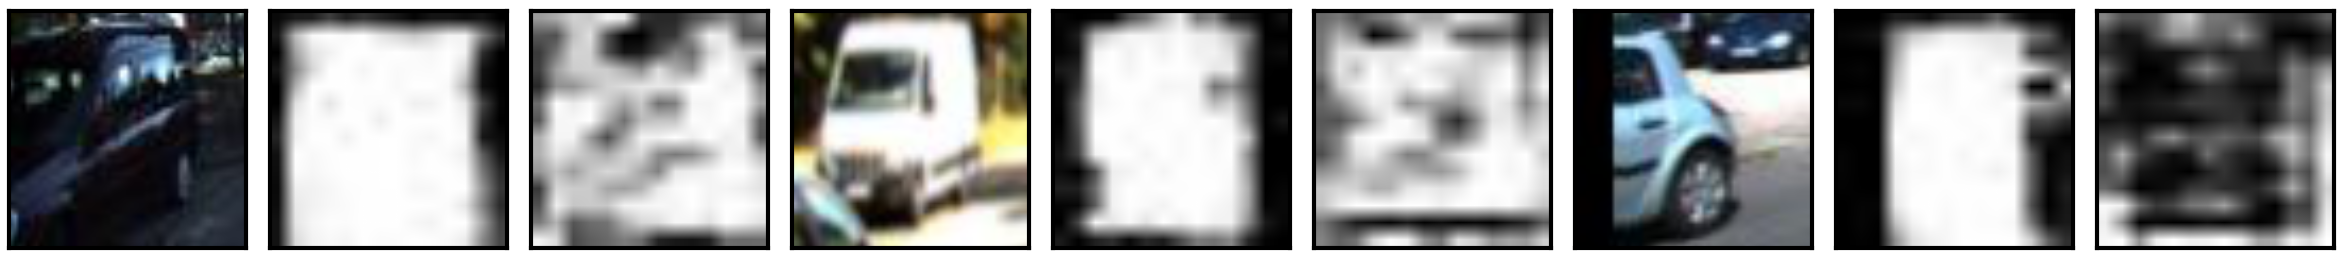
\includegraphics[width=\textwidth]{soft_att}
%    \vspace{.1\baselineskip}
   \caption*{\large Left to right: glimpses and segmentations learned with and without appearance loss.
   Attention loss leads to distractor suppression.} 
\end{minipage}